%% Beginning of file 'sample631.tex'
%%
%% Modified 2021 March
%%
%% This is a sample manuscript marked up using the
%% AASTeX v6.31 LaTeX 2e macros.
%%
%% AASTeX is now based on Alexey Vikhlinin's emulateapj.cls 
%% (Copyright 2000-2015).  See the classfile for details.

%% AASTeX requires revtex4-1.cls and other external packages such as
%% latexsym, graphicx, amssymb, longtable, and epsf.  Note that as of 
%% Oct 2020, APS now uses revtex4.2e for its journals but remember that 
%% AASTeX v6+ still uses v4.1. All of these external packages should 
%% already be present in the modern TeX distributions but not always.
%% For example, revtex4.1 seems to be missing in the linux version of
%% TexLive 2020. One should be able to get all packages from www.ctan.org.
%% In particular, revtex v4.1 can be found at 
%% https://www.ctan.org/pkg/revtex4-1.

%% The first piece of markup in an AASTeX v6.x document is the \documentclass
%% command. LaTeX will ignore any data that comes before this command. The 
%% documentclass can take an optional argument to modify the output style.
%% The command below calls the preprint style which will produce a tightly 
%% typeset, one-column, single-spaced document.  It is the default and thus
%% does not need to be explicitly stated.
%%
%% using aastex version 6.3
\documentclass[twocolumn]{aastex631}

%% The default is a single spaced, 10 point font, single spaced article.
%% There are 5 other style options available via an optional argument. They
%% can be invoked like this:
%%
%% \documentclass[arguments]{aastex631}
%% 
%% where the layout options are:
%%
%%  twocolumn   : two text columns, 10 point font, single spaced article.
%%                This is the most compact and represent the final published
%%                derived PDF copy of the accepted manuscript from the publisher
%%  manuscript  : one text column, 12 point font, double spaced article.
%%  preprint    : one text column, 12 point font, single spaced article.  
%%  preprint2   : two text columns, 12 point font, single spaced article.
%%  modern      : a stylish, single text column, 12 point font, article with
%% 		  wider left and right margins. This uses the Daniel
%% 		  Foreman-Mackey and David Hogg design.
%%  RNAAS       : Supresses an abstract. Originally for RNAAS manuscripts 
%%                but now that abstracts are required this is obsolete for
%%                AAS Journals. Authors might need it for other reasons. DO NOT
%%                use \begin{abstract} and \end{abstract} with this style.
%%
%% Note that you can submit to the AAS Journals in any of these 6 styles.
%%
%% There are other optional arguments one can invoke to allow other stylistic
%% actions. The available options are:
%%
%%   astrosymb    : Loads Astrosymb font and define \astrocommands. 
%%   tighten      : Makes baselineskip slightly smaller, only works with 
%%                  the twocolumn substyle.
%%   times        : uses times font instead of the default
%%   linenumbers  : turn on lineno package.
%%   trackchanges : required to see the revision mark up and print its output
%%   longauthor   : Do not use the more compressed footnote style (default) for 
%%                  the author/collaboration/affiliations. Instead print all
%%                  affiliation information after each name. Creates a much 
%%                  longer author list but may be desirable for short 
%%                  author papers.
%% twocolappendix : make 2 column appendix.
%%   anonymous    : Do not show the authors, affiliations and acknowledgments 
%%                  for dual anonymous review.
%%
%% these can be used in any combination, e.g.
%%
%% \documentclass[twocolumn,linenumbers,trackchanges]{aastex631}
%%
%% AASTeX v6.* now includes \hyperref support. While we have built in specific
%% defaults into the classfile you can manually override them with the
%% \hypersetup command. For example,
%%
%% \hypersetup{linkcolor=red,citecolor=green,filecolor=cyan,urlcolor=magenta}
%%
%% will change the color of the internal links to red, the links to the
%% bibliography to green, the file links to cyan, and the external links to
%% magenta. Additional information on \hyperref options can be found here:
%% https://www.tug.org/applications/hyperref/manual.html#x1-40003
%%
%% Note that in v6.3 "bookmarks" has been changed to "true" in hyperref
%% to improve the accessibility of the compiled pdf file.
%%
%% If you want to create your own macros, you can do so
%% using \newcommand. Your macros should appear before
%% the \begin{document} command.
%%
\newcommand{\vdag}{(v)^\dagger}
\newcommand\aastex{AAS\TeX}
\newcommand\latex{La\TeX}

\newcommand{\racomment}[1]{{\color{blue}#1}}
\newcommand{\dycomment}[1]{{\color{purple}#1}}

%% Reintroduced the \received and \accepted commands from AASTeX v5.2
%\received{March 1, 2021}
%\revised{April 1, 2021}
%\accepted{\today}

%% Command to document which AAS Journal the manuscript was submitted to.
%% Adds "Submitted to " the argument.
%\submitjournal{PSJ}

%% For manuscript that include authors in collaborations, AASTeX v6.31
%% builds on the \collaboration command to allow greater freedom to 
%% keep the traditional author+affiliation information but only show
%% subsets. The \collaboration command now must appear AFTER the group
%% of authors in the collaboration and it takes TWO arguments. The last
%% is still the collaboration identifier. The text given in this
%% argument is what will be shown in the manuscript. The first argument
%% is the number of author above the \collaboration command to show with
%% the collaboration text. If there are authors that are not part of any
%% collaboration the \nocollaboration command is used. This command takes
%% one argument which is also the number of authors above to show. A
%% dashed line is shown to indicate no collaboration. This example manuscript
%% shows how these commands work to display specific set of authors 
%% on the front page.
%%
%% For manuscript without any need to use \collaboration the 
%% \AuthorCollaborationLimit command from v6.2 can still be used to 
%% show a subset of authors.
%
%\AuthorCollaborationLimit=2
%
%% will only show Schwarz & Muench on the front page of the manuscript
%% (assuming the \collaboration and \nocollaboration commands are
%% commented out).
%%
%% Note that all of the author will be shown in the published article.
%% This feature is meant to be used prior to acceptance to make the
%% front end of a long author article more manageable. Please do not use
%% this functionality for manuscripts with less than 20 authors. Conversely,
%% please do use this when the number of authors exceeds 40.
%%
%% Use \allauthors at the manuscript end to show the full author list.
%% This command should only be used with \AuthorCollaborationLimit is used.

%% The following command can be used to set the latex table counters.  It
%% is needed in this document because it uses a mix of latex tabular and
%% AASTeX deluxetables.  In general it should not be needed.
%\setcounter{table}{1}

%%%%%%%%%%%%%%%%%%%%%%%%%%%%%%%%%%%%%%%%%%%%%%%%%%%%%%%%%%%%%%%%%%%%%%%%%%%%%%%%
%%
%% The following section outlines numerous optional output that
%% can be displayed in the front matter or as running meta-data.
%%
%% If you wish, you may supply running head information, although
%% this information may be modified by the editorial offices.
\shorttitle{\textit{Roman} Exoplanet Astrometry}
\shortauthors{Yahalomi et al.}
%%
%% You can add a light gray and diagonal water-mark to the first page 
%% with this command:
%% \watermark{text}
%% where "text", e.g. DRAFT, is the text to appear.  If the text is 
%% long you can control the water-mark size with:
%% \setwatermarkfontsize{dimension}
%% where dimension is any recognized LaTeX dimension, e.g. pt, in, etc.
%%
%%%%%%%%%%%%%%%%%%%%%%%%%%%%%%%%%%%%%%%%%%%%%%%%%%%%%%%%%%%%%%%%%%%%%%%%%%%%%%%%
\graphicspath{{./}{figures/}}
%% This is the end of the preamble.  Indicate the beginning of the
%% manuscript itself with \begin{document}.
\begin{document}

\title{Optimizing an Observing Plan for \textit{Roman} Astrometry of \linebreak Terra Hunting Stars to Determine P(Jupiter $|$ Earth)}

%% LaTeX will automatically break titles if they run longer than
%% one line. However, you may use \\ to force a line break if
%% you desire. In v6.31 you can include a footnote in the title.

%% A significant change from earlier AASTEX versions is in the structure for 
%% calling author and affiliations. The change was necessary to implement 
%% auto-indexing of affiliations which prior was a manual process that could 
%% easily be tedious in large author manuscripts.
%%
%% The \author command is the same as before except it now takes an optional
%% argument which is the 16 digit ORCID. The syntax is:
%% \author[xxxx-xxxx-xxxx-xxxx]{Author Name}
%%
%% This will hyperlink the author name to the author's ORCID page. Note that
%% during compilation, LaTeX will do some limited checking of the format of
%% the ID to make sure it is valid. If the "orcid-ID.png" image file is 
%% present or in the LaTeX pathway, the OrcID icon will appear next to
%% the authors name.
%%
%% Use \affiliation for affiliation information. The old \affil is now aliased
%% to \affiliation. AASTeX v6.31 will automatically index these in the header.
%% When a duplicate is found its index will be the same as its previous entry.
%%
%% Note that \altaffilmark and \altaffiltext have been removed and thus 
%% can not be used to document secondary affiliations. If they are used latex
%% will issue a specific error message and quit. Please use multiple 
%% \affiliation calls for to document more than one affiliation.
%%
%% The new \altaffiliation can be used to indicate some secondary information
%% such as fellowships. This command produces a non-numeric footnote that is
%% set away from the numeric \affiliation footnotes.  NOTE that if an
%% \altaffiliation command is used it must come BEFORE the \affiliation call,
%% right after the \author command, in order to place the footnotes in
%% the proper location.
%%
%% Use \email to set provide email addresses. Each \email will appear on its
%% own line so you can put multiple email address in one \email call. A new
%% \correspondingauthor command is available in V6.31 to identify the
%% corresponding author of the manuscript. It is the author's responsibility
%% to make sure this name is also in the author list.
%%
%% While authors can be grouped inside the same \author and \affiliation
%% commands it is better to have a single author for each. This allows for
%% one to exploit all the new benefits and should make book-keeping easier.
%%
%% If done correctly the peer review system will be able to
%% automatically put the author and affiliation information from the manuscript
%% and save the corresponding author the trouble of entering it by hand.


\correspondingauthor{Daniel A. Yahalomi}
\email{daniel.yahalomi@columbia.edu}

\author[0000-0003-4755-584X]{Daniel A. Yahalomi} 
\affiliation{Department of Astronomy, Columbia University, 550 W 120th St., New York NY 10027, USA}


\author[0000-0002-5151-0006]{David N. Spergel}
\affiliation{Center for Computational Astrophysics, Flatiron Institute, 162 5th Avenue, New York, NY 10010, USA}

\author[0000-0003-4540-5661]{Ruth Angus}
\affiliation{American Museum of Natural History, Central Park West, Manhattan, NY, USA}
\affiliation{Center for Computational Astrophysics, Flatiron Institute, 162 5th Avenue, New York, NY 10010, USA}
\affiliation{Department of Astronomy, Columbia University, 550 W 120th St., New York NY 10027, USA}






%% Note that the \and command from previous versions of AASTeX is now
%% depreciated in this version as it is no longer necessary. AASTeX 
%% automatically takes care of all commas and "and"s between authors names.

%% AASTeX 6.31 has the new \collaboration and \nocollaboration commands to
%% provide the collaboration status of a group of authors. These commands 
%% can be used either before or after the list of corresponding authors. The
%% argument for \collaboration is the collaboration identifier. Authors are
%% encouraged to surround collaboration identifiers with ()s. The 
%% \nocollaboration command takes no argument and exists to indicate that
%% the nearby authors are not part of surrounding collaborations.

%% Mark off the abstract in the ``abstract'' environment. 
\begin{abstract}

Earth-mass planets on year-long orbits and gas giants on decade-long orbits lie at the edge of current detection limits. The \textit{Nancy Grace Roman Space Telescope}, scheduled to launch in late 2025, will be capable of precision astrometry using its wide field imager. For bright stars, \textit{Roman} may be able to achieve astrometric accuracy of 1-10 $\mu$as. By combining measurements from a \textit{Roman} astrometry observing program with Gaia data we can increase the baseline of astrometric observations in order to recover planets on wide, Jupiter-like orbits. The Terra Hunting Experiment (THE), starting in 2022, will take nightly radial velocity (RV) observations of at least 40 bright G and K dwarfs for 10 years, in search of planets that are Earth-like in mass and temperature. Together, \textit{Roman} and THE may be capable of detecting both Earth-analogues and Jupiter-analogues. In order to design and optimize an observing strategy for \textit{Roman} astrometry, we simulate a set of possible planetary signals both in single and multi-planet systems, based on planetary architecture and stability models. Jupiter has played a significant dynamical role in our own Solar system, and the occurrence rate of outer Jovian planets in systems with terrestrial planets could inform planet formation and dynamical evolution models. We describe an observing plan that could provide estimates on P(Jupiter $\vert$ Earth), the probability that a star has a Jupiter analogue, given that it has an Earth analogue.

% If you start each new sentence on a separate line in your text editor, 
% you'll find it easier to edit later on -- you'll be able to comment out entire
% sentences at once, for example. 

\end{abstract}

%% Keywords should appear after the \end{abstract} command. 
%% The AAS Journals now uses Unified Astronomy Thesaurus concepts:
%% https://astrothesaurus.org
%% You will be asked to selected these concepts during the submission process
%% but this old "keyword" functionality is maintained in case authors want
%% to include these concepts in their preprints.
\keywords{}

%% From the front matter, we move on to the body of the paper.
%% Sections are demarcated by \section and \subsection, respectively.
%% Observe the use of the LaTeX \label
%% command after the \subsection to give a symbolic KEY to the
%% subsection for cross-referencing in a \ref command.
%% You can use LaTeX's \ref and \label commands to keep track of
%% cross-references to sections, equations, tables, and figures.
%% That way, if you change the order of any elements, LaTeX will
%% automatically renumber them.
%%
%% We recommend that authors also use the natbib \citep
%% and \citet commands to identify citations.  The citations are
%% tied to the reference list via symbolic KEYs. The KEY corresponds
%% to the KEY in the \bibitem in the reference list below. 

\section{Introduction} \label{sec:intro}


The detection and study of extrasolar planets (exoplanets) has a long history of exciting and surprising discoveries. Astronomers have detected worlds vastly different than those in our own solar system \racomment{: `zombie' planets orbiting a pulsar \citep{Wolszczan1992}, so called hot Jupiters or gas giants orbiting a star at shorter than 10 day periods \citep{Latham1989, Mayor1995}, planets orbiting main sequence binary star systems \citep{Correia2005}, \textbf{(...other exotic planet types)} -- nice but not necessary}. However, despite all this progress in the field of exoplanets, astronomers have yet to detect true Solar system analogs. This has been driven by observational detection limits, as both Earth-mass objects on year-long orbits and gas-giant planets on 10 year (Jupiter-like) or longer orbits lie outside of current telescope capabilities. Figure \ref{fig: demographics} shows the current exoplanet detections as well as the Earth and Jupiter in mass vs. period space.
\racomment{Always explain a figure in the text and hammer the point home. What point is figure 1 illustrating and how?}

In the coming decade, with radial velocity surveys designed for the purpose of Earth-twin detection \citep{Hall2018} and with astrometric observations from space missions like \textit{Gaia}, which will release astrometry in data release 4 (DR4) \citep{Gaia2016} and \textit{The Nancy Grace Roman}, set to launch in late 2025 \citep{Spergel2015}, there is promise in the detection of Solar System analogs. While it has been demonstrated that \textit{Roman} will contribute heavily to exoplanet science via the microlensing method \citep{Penny2019, Johnson2020}, it will also be capable of high precision astrometric exoplanet detection \citep{Sanderson2019}. Astrometric observations complement radial velocity surveys targeting Earth-analogs in that (1) astrometric measurements can break the mass-inclination degeneracy inherant in radial velocity observations, (2) astrometric measurements, which are more sensitive to longer periods, complement RV observations, which are more sensitive to shorter periods, and (3) astrometric observation could allow us to marginalize over stellar noise in the RV data as astrometry is less sensitive to stellar noise than the Doppler method.
\racomment{Great!}
The detection capabilities of astrometric surveys drop very steeply when the period of the orbit extends past the duration of the astrometric observations \citep{Casertano2008}. Thus, in targeting planets on long orbits with astrometry, combining observations from \textit{Gaia} and \textit{Roman} will be critical in extending the period baseline for detection capabilities. 

\begin{figure}[htb] \label{fig: demographics}
    \centering 
    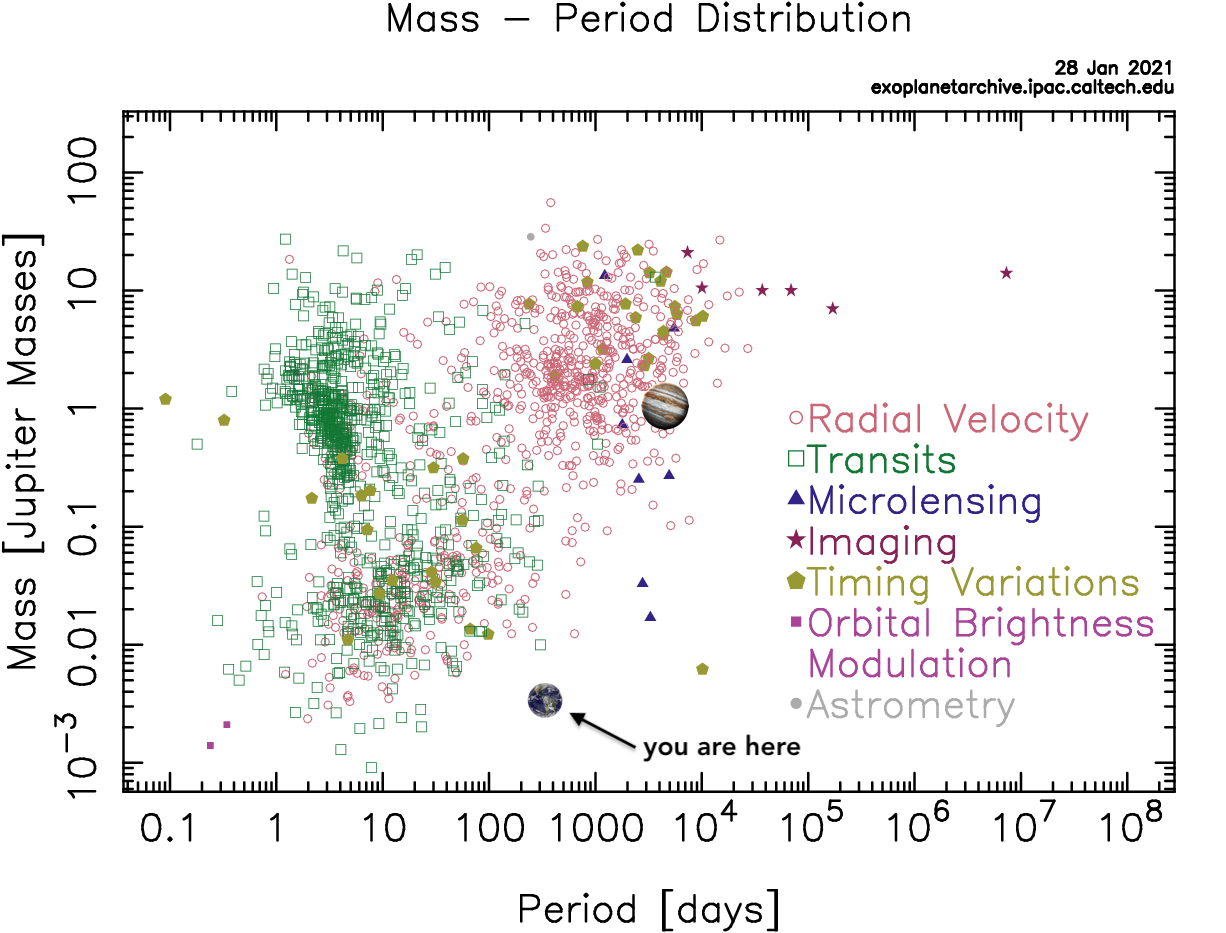
\includegraphics[width=\columnwidth]{exo_massperiod_wEarthJupiter.png}
    \caption{Mass vs. \racomment{orbital} period of confirmed exoplanets and the method of detection. Earth and Jupiter are also plotted. The paucity of planets at low masses and long periods reflects the limitations of our observational techniques rather than true exoplanet demographics.. Demographics figure generated with tools from \href{exoplanetarchive.ipac.caltech.edu}{exoplanetarchive.ipac.caltech.edu}.}
\end{figure}


The formation and migration of gas giant planets and the interactions between gas giants in our Solar System have played a critical role in the characteristics of the planets in our Solar System \citep{Tsiganis2005, Morbidelli2005, Gomes2005, Walsh2011, Batygin2015}. Further, Jupiter may have played a crucial role in Earth's habitability, in that it (1) helps stabilize Earth's orbit and thus climate and (2) it shields Earth from possibly devastating impacts \citep{Raymond2004} \textbf{would like another resource here}. As the Earth is the only presently known habitable planet, it is natural to search for Earth-twins in pursuit of habitable planets. Further, if Jupiter (and Saturn) have played such an important role both in the formation, stability, and habitability of Earth, it is also of interest to search for Earth-analogues with external gas giant planets. Thus, in order to better understand the demographics of Earth-analogues, an important question to investigate is the percentage of Earth-analogues that also have Jupiter-like (or Saturn-like) companions.
\racomment{Very well explained.}

In this paper, we present an observing strategy with \textit{Roman} astrometry, capable of detecting both Earth-analogues and Jupiter-analogues around Terra Hunting Stars. By combining observations from the Terra Hunting Doppler survey with \textit{Gaia} and \textit{Roman} astrometry, we can investigate the probability that a \racomment{S}olar-type star has an orbiting Jupiter-like planet, given that the \racomment{S}olar-type star has an orbiting Earth-like planet ($P(\textrm{Jupiter} | \textrm{Earth})$). Specifically, in this proposed \textit{Roman} observing strategy, we will obtain follow-up astrometric observations of stars that show radial velocity signals consistent with an Earth-analogue via the Terra Hunting Experiment. 

In combination with exoplanet demographic models, one could then infer, using Bayes theory, the probability that a Solar-type star has an orbiting Earth-like planet, given that the star has an orbiting Jupiter-like planet ($P(\textrm{Earth} | \textrm{Jupiter})$), by using the Equation \ref{eq: Bayes}.

\begin{equation} \label{eq: Bayes}
    P(\textrm{Earth} | \textrm{Jupiter}) = \frac{P(\textrm{Jupiter} | \textrm{Earth}) \, P(\textrm{Earth})} {P(\textrm{Jupiter})}
\end{equation}

This version of the equation has the inherent benefit, in that it is easier to detect Jupiter analogues, as they are so much more massive than Earth-like planets, and thus have a larger gravitational effect on their host star. However, this version of the equation has the downside in that the model would be built on assumptions of P(Earth) and P(Jupiter).

To date, similar studies have been conducted for super-Earths and cold-Jupiters \citep{Zu2018, Masuda2020} as well as for hot-Jupiters and cold-Jupiters \citep{Knutson2014}. \citet{Zu2018} investigated the relations between inner ($<$ 1 AU) super-Earths and outer ($>$ 1 AU) cold-Jupiters and determined P(\textrm{cold-Jupiter}$|$\textrm{super-Earth}) $\sim$ 30 $\%$. By comparing this value with results from \citet{Cumming2008}, which predicts that 10$\%$ of Sun-like stars should have at least one cold-Jupiter, they determined that cold-Jupiters appear three times more often around super-Earth hosts than around Sun-like stars. Finally, by arguing that P(\textrm{super-Earth}) = 30$\%$ and using a version of Bayes theorem as shown in Equation \ref{eq: Bayes}, \citet{Zu2018} argued that P(\textrm{super-Earth}$|$\textrm{cold-Jupiter}) $\sim$ 90$\%$. Subsequently, \citet{Masuda2020} showed that stellar systems with super-Earths and cold-Jupiters tend to be coplanar, but not quite as coplanar as the Solar System. Due to this and the strong association between the fraction of Sun-like stars that have both a cold-Jupiter and a super-Earth, they suggest that this provides a ``clue'' about the formation and evolution of these systems. \citet{Knutson2014} conducted a radial velocity study in search for long-period companions to inner hot-Jupiters and found that in their sample of 51 systems, 51$\%$ $\pm$ 10$\%$ of the systems had outer companions with masses between 1–13 M$_{\textrm{Jup}}$ and orbital semi-major axes between 1–20 AU.
\racomment{Great review! Perhaps add a take-home statement here and frame a question that you would like to answer with Roman \& THE?}

\section{Background, Missions, and Equations}

\racomment{I suggest making mission backgrounds part of the introduction and moving equations to the methods section.}

\subsection{\textit{Nancy Grace Roman Space Telescope}}

The \textit{Nancy Grace Roman Space Telescope} is set to launch in 2025. \textit{Roman} will be used to investigate many interesting and important topics in astronomy, such as studies of dark energy and dark matter, exoplanet detection and imaging, and a wide range of infrared astrometry. \textit{Roman} will have a 2.4m primary lens, which is the same size as the \textit{Hubble Space Telescope}, but a viewing window 100 times larger than \textit{Hubble}. \textit{Roman} will have no proprietary time and all observing time will be competed via external proposals. \textit{Roman} has a five-year primary mission length.

As previously mentioned, \textit{Roman} is expected to detect thousands of exoplanet microlensing events, which will be crucial in expanding the baseline of period sensitivity in exoplanet detection and improving our understanding of long period exoplanets \citep{Penny2019, Johnson2020}. However, the microlensing method only provides for a single observation of a planetary system. \textit{Roman} will also be capable of high precision astrometry and will provide at least a factor of three improvement over the current state of the art astrometric observations in this wavelength range. Further, \textit{Roman} astrometry of bright nearby stars ($<$ 10 pc) could detect Earth-mass exoplanets in some cases in the habitable zone, as well as more distant planets with periods up to $>$10 years by adding earlier astrometric observations from \textit{Gaia} \racomment{(citations)}.
It is estimated that \textit{Roman} will be capable of astrometric precision of $\sim$ 1-10 $\mu$as \citep{Sanderson2019}. 

As the stars we would like to observe are very bright, exoplanet astrometry with \textit{Roman} can be pursued using two different methods, in order to avoid saturation:
\begin{enumerate}

    \item \textbf{Diffraction Spike Method:} In the diffraction spike method, observations are centered on the detector's diffraction spike. This is possible as \textit{Roman} uses H4RG detectors rather than CCDs, in which pixels bleed into nearby pixels when saturated. Measurement accuracy with this method will likely be limited by systematics, and so it is ideal to take multiple observations of a system to reduce uncertainties \citep{Sanderson2019}. \citet{Melchior2018} investigated the capabilities of a \textit{Roman} dedicated guest observing plan using the diffraction spike method for detection of Earth-mass exoplanets. In the paper, they argued that \textit{Roman} astrometry using the diffraction spike method could obtain 10 $\mu$as astrometric observations with a single 100s exposure for a R=6 or a J=5 star -- precise enough to detect Earth-mass exoplanets on $\geq$ 1 year orbits around stars within a few pc.
    
    \item \textbf{Spatial Scanning Method:} In the spatial scanning method, as the name suggests, the telescope is slowly slewed in a specific direction during the observation. This creates spatial tracks for the brighter stars and allows for the observation of reference stars in the same field. In so doing, this observational technique avoids saturation by spreading the signal over hundreds, or even thousands, of pixels -- and thus allows for orders of magnitude of more photons. Subsequent spacial scans in two perpendicular directions allows for three-dimensional high precision observations. Similarly to the diffraction spike method, measurement accuracy with spatial scanning will likely be limited by systematics, and so it is ideal to take multiple observations of a system to reduce uncertainties \citep{Sanderson2019}. This method has been applied to \textit{Hubble} observations, in observing bright Cepheids with astrometric precision of 20-40 $\mu$as \citep{Riess2014}.
    \racomment{Very clear!}

\end{enumerate}


\subsection{Terra Hunting Experiment}
The HARPS3 will be a fibre fed, high resolution, high stability, echelle spectrograph. The HARPS3 instrument will be installed on the 2.5m Isaac Newton Telescope in La Palma in the Canary Islands \citep{Thompson2016, Hall2016}. HARPS3 will be a close-copy to HARPS \citep{Mayor2003, Rupprecht2004} and HARPS-North \citep{Cosentino2012}. The Terra Hunting Experiment (THE) will be conducted on HARPS3. THE aims to discover Earth-twins via 10-years of daily observations of at least 40 bright nearby Sun-like stars. By combining the high precision of HARPS3 with the radical observation plan of THE, observers have the greatest chance at detecting low mass, long period exoplanets.
In fact, it has been shown that THE can detect Earth-twins in the habitable zone of Solar-type stars, for both single and multi-planet systems and with stellar signals \citep{Hall2018}.
Further, simulations have suggested that THE can outperform a typical reference survey and preforms comparably to an uninterrupted space-based schedule on accuracy of recovered parameters for Earth-twin detection \citep{Hall2018}. 


\subsection{\textit{Gaia}}
\textit{Gaia} is a space-based telescope with the mission to chart a three-dimensional map of the Milky Way, in pursuit of understanding the formaiton, composition, and evolution of the Milky Way. \textit{Gaia}, which launched in 2013, had a nominal mission length of 5 years, but it has been extended through 2022 with an possible extension through 2025. \textit{Gaia} will release astrometric observation in an upcoming data release, and is expected to have a significant impact on the knowledge of both exoplanet demographics and physical properties. The utility of \textit{Gaia} for exoplanet detection and characterization via the astrometric method has been well studied, and current models and simulations predict the detection of $\sim$21,000 exoplanets for a 5 year mission \citep{Bernstein1995, Casertano1996, Casertano2008, Perryman2014, Ranalli2018}. By combining astrometric data from \textit{Gaia} and \textit{Roman} we can extend the baseline of observations, thus extending sensitivity to period up to and potentially beyond 10 years.



\racomment{It would be good to add a bit more of a project overview before you start describing technical details.
Describe what kinds of planetary systems you'll simulate and why this will help answer the question.}

\racomment{I suggest making a new section called methods which starts with an overview of what kind of planetary systems you're going to simulate, then introduces modeling methods with technical details. I would probably put the equations before the description of sampling methods: exoplanet and PyMC3.}

\clearpage

\section{Methods}
\subsection{\textit{exoplanet} Code}
For both simulating the orbits of the planets sampled in our paper and efficiently modeling the subsequent orbits, we use the \textit{exoplanet} codebase. \textit{exoplanet} is an open source toolkit that uses efficient gradient based sampling to model exoplanet data from transits, radial velocities, and/or astrometry \citep{Foreman-Mackey2021}. Practically, in its gradient-based inference, \textit{exoplanet} uses methods such as Hamiltonian Monte-Carlo \citep{}, No U-Turn Sampling \citep{}, and variational inference \citep{}, which can improve performance (especially when there are more than 10 parameters) by orders of magnitude vs. other modeling methods such as Markov-Chain Monte Carlo (MCMC) \citep{Foreman-Mackey2021}. In contrast to many other tools in the vast ecosystem of exoplanet and time domain modeling software, \textit{exoplanet} is designed as a framework with which a pipeline can be generated -- rather than a finished code base with a ``push go'' button \citep{Foreman-Mackey2021}. \textit{exoplanet} uses PyMC3, a model building language and inference engine that scales well in the many parameter regime \citep{Salvatier2016}. 



In brief, given a set of orbital parameters, a cadence of observations, a duration of observations, and assuming an error, we can create a simulated dataset of both radial velocity and astrometry observations for a single exoplanet. We then model this simulated data using \textit{exoplanet} and determine whether these orbital parameters can be accurately recovered. See Figure \ref{fig: schematic} for a schematic of this process.





\begin{figure*}[htb] \label{fig: schematic}
    \centering 
    \includegraphics[width=\textwidth]{schematic.pdf}
    \caption{Schematic of process from orbital parameters, to simulated data, to final predictions.}
\end{figure*}


\subsection{Simulating Earth and Jupiter analogues}
\dycomment{Add to section about simulating data, will do so once more concrete on simulated planetary parameters.}
\linebreak 
We use \textit{exoplanet} to simulate both the theoretical radial velocity and astrometric signals. For the radial velocity data, we adopt THE's nightly cadence and 10 year duration, as described in \citet{Hall2018} while for the astrometric simulated data, we chose a cadence and duration of observations. We then introduce random gaussian noise to both the radial velocity and astrometry signals -- producing our simulated dataset. 



\subsection{Modeling Pipeline}
\subsubsection{Radial Velocity Model}
We then sample the parameter space using gradient-based MCMC with \textit{exoplanet} for the three simulated planetary populations (Earth-like only, Jupiter-like only, and Earth-like and Jupiter-like) around Solar mass and radius stars. We adopted the expected precision of the THE radial velocity and \textit{Roman} astrometric observations, placing Gaussian uncertainties on the data points with the same standard deviation as the those used to simulate the data ($\sigma_{\textrm{RV}} = 0.01$ m/s, $\sigma_{\rho} = 0.001 ''$, $\sigma_{\theta} = 0.1$ rad). First, we fit a radial velocity only model, in order to initially sample the parameter space without mass-inclination determination. We sample period (P), eccentricity (e), argument of the periapsis of the star ($\omega$), radial velocity semi-amplitude (K), and the time of transit (T$_0$). As is standard in MCMC modeling of exoplanet radial velocity data, we sampled the eccentricity and argument of periapsis as $\sqrt{\textrm{e}}\cos{\omega}$ and $\sqrt{\textrm{e}}\sin{\omega}$ \dycomment{(cite exofast, others?)}. Additionally, we sampled period and semi-amplitude in natural logarithmic space. The five radial velocity modeling parameters, priors, and starting points can be seen in Table \ref{table: rv_params}. 

\begin{table} 
\centering
\caption{Parameters for the Radial Velocity MCMC Model}
\label{table: rv_params}
\begin{tabular}{ c  c  c }
\hline
Parameter & Prior\footnote{\label{fn: priorLC} Priors adopted in the MCMC model. $\mathcal{U}(x,y)$ denotes a uniform distribution between x and y. $\mathcal{N}(\mu, \sigma^2$) denotes a Gaussian distribution centered at $\mu$ with a standard deviation of $\sigma$.} & Starting Point\\
\hline 

$\log \textrm{P}$  & $\mathcal{N}(\log \textrm{P_0}$, $\sigma_{P_0}^2$) &  $\log \textrm{P_0}$ \\
$\log \textrm{K}$  & $\mathcal{N}(\log \textrm{K_0}$, $5^2$) & $\log \textrm{K_0}$  \\
$\sqrt{\textrm{e}}\cos{\omega}$ & $\mathcal{U}$(0, 1) & 0.01  \\
$\sqrt{\textrm{e}}\sin{\omega}$ & $\mathcal{U}$(0, 1) & 0.01  \\
T$_0$ & $\mathcal{N}$(T$_{0,0}$, $\sigma_{\textrm{T}_{0,0}}^2$) & T$_{0,0}$  \\

\hline
\end{tabular}
\end{table}


In modeling the simulated data, we followed the standard Keplerian equations. Including the magnitude of barycentric motion of the star ($\gamma$), which we set to zero as it is just a constant, the radial velocity signal is described by:

\begin{equation} \label{eq: RVsignal}
    RV(\nu) = K \Big[\cos \big(\nu(t) + \omega \big) + e \cos \omega \Big] + \gamma
\end{equation}

where

\begin{equation} \label{eq: semi-amplitude}
    K = (\frac{2\pi G}{P})^{\frac{1}{3}} \frac{\textrm{M}_{p} \sin{i}}{\textrm{m}_{*}^\frac{2}{3}} \frac{1}{\sqrt{1-e^2}}
\end{equation}


\dycomment{I am confused by the treatment of true anomaly, mean anomaly, and eccentric anomaly as used by \textit{exoplanet} and the exact process used to solve Kepler's equations. In the paper, they mention ``In practice, we have found it more efficient to fuse the calculations of the eccentric anomaly E and the true anomaly f working only with the sine and cosines of these quantites.'' I need to look more into this and then complete this section}

\subsubsection{Radial Velocity and Astrometric Model}
Now that we have a sense of the radial velocity parameter space, we can include the astrometric data and model, and jointly sample radial velocity and astrometric parameter space using both simulated datasets in order to recover a complete posterior sample. As we are testing different astrometric observational cadences and durations, modeling the RV observations independently first has the added benefit of speeding up the astrometric modeling. By using the RV fit as a starting point for the joint MCMC, for all parameters besides the longitude of the ascending node ($\Omega$) and splitting the mass-inclination degeneracy (m$_\textrm(p)$ and i), we can more efficiently model the larger parameter space. We adopt the median parameters from the RV MCMC fit as the starting points in the joint fit MCMC and place Gaussian priors on three of the five orbital parameters (P, K, and T$_0$) with standard deviations equal to the RV MCMC standard deviations. The complete set of modeled parameters, priors, and starting points for the joint radial velocity and astrometric model can be seen in Table \ref{table: joint_params}.


\begin{table} 
\centering
\caption{Parameters for the Joint Radial Velocity and Astrometric MCMC Model}
\label{table: joint_params}
\begin{tabular}{ c  c  c }
\hline
Parameter & Prior\footnote{\label{fn: priorLC} Priors adopted in the MCMC model. $\mathcal{U}(x,y)$ denotes a uniform distribution between x and y. $\mathcal{N}(\mu, \sigma^2$) denotes a Gaussian distribution centered at $\mu$ with a standard deviation of $\sigma$.} & Starting Point\\
\hline 

$\log \textrm{P}$  & $\mathcal{N}(\log \textrm{P_\textrm{RV}}$, $\sigma_{P_\textrm{RV}}^2$) &  $\log \textrm{P_\textrm{RV}}$ \\
$\log \textrm{K}$  & $\mathcal{N}(\log \textrm{K_\textrm{RV}}$, $\sigma_\textrm{RV}^2$) & $\log \textrm{K_\textrm{RV}}$  \\
$\sqrt{\textrm{e}}\cos{\omega}$ & $\mathcal{U}$(0, 1) & $\sqrt{\textrm{e}}\cos{\omega}_\textrm{RV}$  \\
$\sqrt{\textrm{e}}\sin{\omega}$ & $\mathcal{U}$(0, 1) & $\sqrt{\textrm{e}}\sin{\omega}_\textrm{RV}$  \\
T$_0$ & $\mathcal{N}$(T$_{0,\textrm{RV}}$, $\sigma_{\textrm{T}_{0,\textrm{RV}}}^2$) & T$_{0,\textrm{RV}}$  \\
m$_\textrm{p}$ & $\mathcal{U}$(0, 30) M$_\Earth$ & ...  \\
i & $\mathcal{U}$(0, $\pi$/2) & ...  \\
$\Omega$ & $\mathcal{U}$(-$\pi$, $\pi$) & ... \\

\hline
\end{tabular}
\end{table}



In modeling the astrometric data, we used the following astrometric equations, which are built into \textit{exoplanet}. Including both parallax and proper motion, the total astrometric signal is described by 


\begin{equation} \label{eq: astrometric_xi}
   \xi (t) = \alpha_0^\star + \pi_{\alpha^\star}{\pi} + (t - t_0)\mu_{\alpha^\star} + B \, X(t) + G \, Y(t)
\end{equation}
\begin{equation}
    \eta (t) = \delta_0 + \pi_{\delta}{\pi} + (t - t_0)\mu_{\delta} + A \, X(t) + F \, Y(t)
\end{equation}    

where $\alpha_{\star} = \alpha \cos \delta$, $(\alpha_0^\star, \delta_0)$ is the refernece right ascension and declination of the star, ($\pi_{\alpha^\star}, \pi_{\delta}$) is the parallax factors describing the parallactic ellipse of the star, and ($\mu_{\alpha^\star}, \mu_{\delta}$) is the proper motion vector of the star. The equation above is parametrized by the Thiele-Innes constants (\dycomment{need to check whether omega values below are for the star or planet}.)

\begin{equation}
    A = \theta (\cos\Omega \cos\omega - \sin\Omega \sin\omega \cos i)
\end{equation}
\begin{equation}
    B = \theta (\sin\Omega \cos\omega + \cos\Omega \sin\omega \cos i)
\end{equation}   
\begin{equation}
    F = \theta (-\cos\Omega \sin\omega - \sin\Omega \cos\omega \cos i)
\end{equation}    
\begin{equation}
    G = \theta (-\sin\Omega \sin\omega + \cos\Omega \cos\omega \cos i)
\end{equation}

where $\theta$ is the semi-major axis of the apparent ellipse or what we will call the astrometric signal due to an orbiting planet. The semi-major axis of the apparent ellipse can be solved using Kepler's Third Law (where m$_{\textrm{tot}}$ is the total mass, or for a single planet system $\textrm{m}_{\textrm{tot}} = \textrm{m}_{\star} + \textrm{m}_{\textrm{p}}$):

\begin{equation}
\theta = [\frac{P^2 \: G \: \textrm{m}_{\textrm{tot}}}{4\pi^2}]^{\frac{1}{3}}
\end{equation}


If we assume a circular orbit and that $\textrm{m}_\textrm{p} \ll \textrm{m}_{\star}$. At a distance ``d'' = $\frac{1}{\pi}$) from the observer and an orbital radius ``R'' = a, the astrometric signal equals...

\begin{equation}
\theta = 
\frac{\textrm{m}_\textrm{p}}{\textrm{m}_{\star}} \frac{\textrm{R}}{\textrm{d}} = 
\Big(\frac{\textrm{G}}{4\pi^2} \Big)^{1/3}  
\frac{\textrm{m}_\textrm{p}}{\textrm{m}_{\star}^{2/3}}
\frac{\textrm{P}^{2/3}}{\textrm{d}}
\end{equation}
\begin{equation}
\theta = 
3 \, \mu \textrm{as} \cdot
\Big(\frac{\textrm{m}_\textrm{p}}{\textrm{M}_{\bigoplus}} \Big)
\Big(\frac{\textrm{m}_\star}{\textrm{M}_{\bigodot}} \Big)^{-2/3}
\Big(\frac{\textrm{P}}{\textrm{yr}} \Big)^{2/3}
\Big(\frac{\textrm{d}}{\textrm{pc}} \Big)^{-1}
\end{equation}

Lastly, (X(t), Y(t)) is the vector describing the motion of the star caused by its planetary orbit. The vector is defined by 

\begin{equation}
X(t) = cos(E(t)) - e
\end{equation}
\begin{equation}
Y(t) = \sqrt{1-e^2} \sin(E(t))
\end{equation}

where E is the eccentric anomaly
\begin{equation}
E = M + e\sin E
\end{equation}

and M is the mean anomaly, which can be determined by a series expansion of the true anomaly and the eccentricity \citep{smart1953}

\dycomment{add series expansion for M.}

\subsection{Synnergies of Astrometric and Radial Velocity Equations}

\dycomment{Add derivation of synnergistic period dependence of astrometry and RV signals}


\begin{figure*}[htb] \label{fig: earth_and_jupiter}
    \centering 
    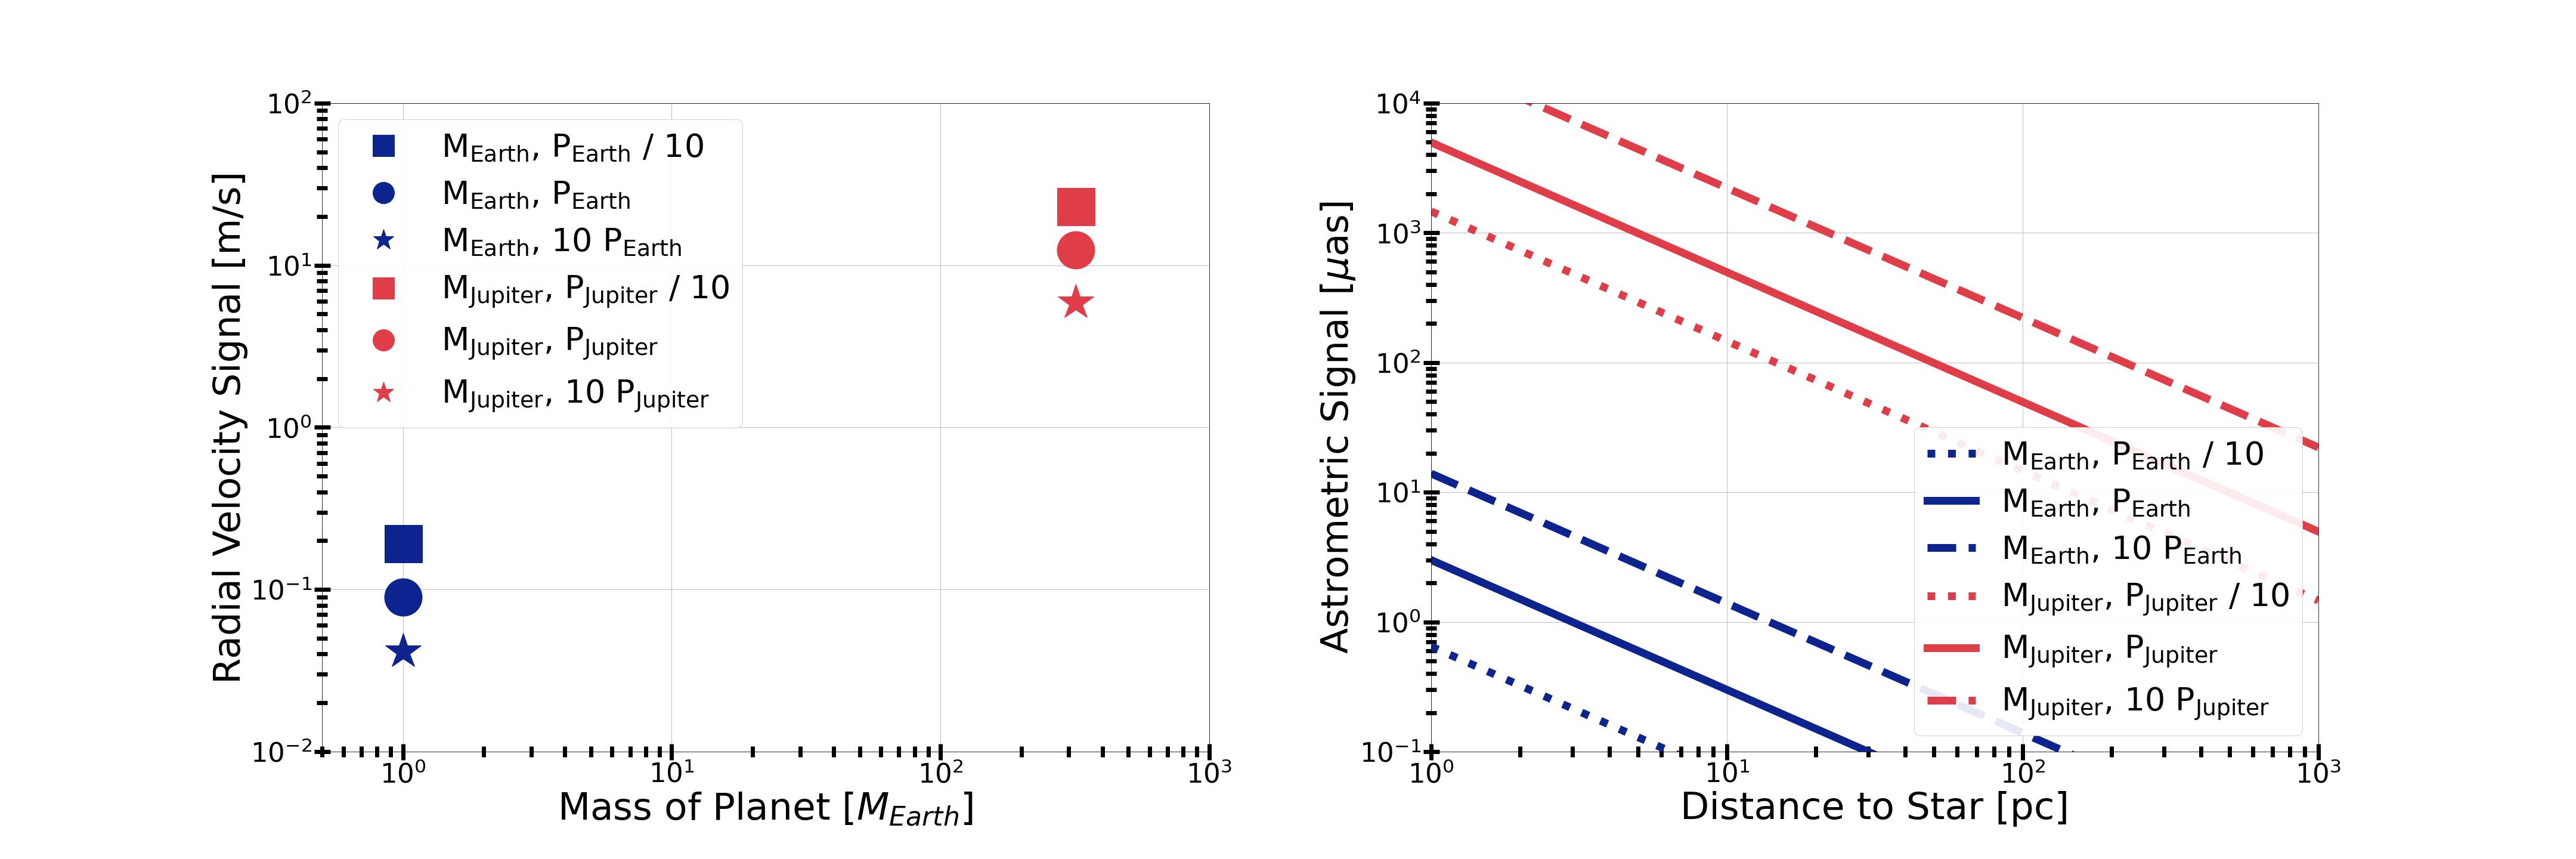
\includegraphics[width=\textwidth]{astometry_and_RV_signal.pdf}
    \caption{Radial velocity and astometric signal for Earth-mass and Jupiter mass objects with periods of 0.1x, 1x, and 10x their solar-system values. RV signal for Earth-mass and Jupiter-mass objects on circular orbits around a Solar mass star. THE is pushing towards 0.1 m/s. (Right) Astrometric signal for Earth-mass and Jupiter-mass objects around Solar mass stars with varying period. Roman astrometry is pushing towards $\sim$1-10 $\mu$as. }
\end{figure*}








%% IMPORTANT! The old "\acknowledgment" command has be depreciated. It was
%% not robust enough to handle our new dual anonymous review requirements and
%% thus been replaced with the acknowledgment environment. If you try to 
%% compile with \acknowledgment you will get an error print to the screen
%% and in the compiled pdf.
\begin{acknowledgments}

\end{acknowledgments}

%% To help institutions obtain information on the effectiveness of their 
%% telescopes the AAS Journals has created a group of keywords for telescope 
%% facilities.
%
%% Following the acknowledgments section, use the following syntax and the
%% \facility{} or \facilities{} macros to list the keywords of facilities used 
%% in the research for the paper.  Each keyword is check against the master 
%% list during copy editing.  Individual instruments can be provided in 
%% parentheses, after the keyword, but they are not verified.

\vspace{5mm}
\facilities{}

%% Similar to \facility{}, there is the optional \software command to allow 
%% authors a place to specify which programs were used during the creation of 
%% the manuscript. Authors should list each code and include either a
%% citation or url to the code inside ()s when available.

\software{}

%% Appendix material should be preceded with a single \appendix command.
%% There should be a \section command for each appendix. Mark appendix
%% subsections with the same markup you use in the main body of the paper.

%% Each Appendix (indicated with \section) will be lettered A, B, C, etc.
%% The equation counter will reset when it encounters the \appendix
%% command and will number appendix equations (A1), (A2), etc. The
%% Figure and Table counter will not reset.

\appendix

\section{Appendix information}


%% For this sample we use BibTeX plus aasjournals.bst to generate the
%% the bibliography. The sample631.bib file was populated from ADS. To
%% get the citations to show in the compiled file do the following:
%%
%% pdflatex sample631.tex
%% bibtext sample631
%% pdflatex sample631.tex
%% pdflatex sample631.tex

\bibliography{main}{}
\bibliographystyle{aasjournal}

%% This command is needed to show the entire author+affiliation list when
%% the collaboration and author truncation commands are used.  It has to
%% go at the end of the manuscript.
%\allauthors

%% Include this line if you are using the \added, \replaced, \deleted
%% commands to see a summary list of all changes at the end of the article.
%\listofchanges

\end{document}

% End of file `sample631.tex'.
